\documentclass[aspectratio=169]{beamer}
\usetheme{Madrid}
\usecolortheme{beaver}
\usefonttheme{serif}
\usepackage{lmodern}

\usepackage[utf8]{inputenc}
\usepackage{graphicx}
\usepackage{pgfplots}
\pgfplotsset{compat=1.18}
\usepackage{amsmath}
\usepackage{url}

\graphicspath{{figures/}}
\setbeamertemplate{frametitle}[default][center]

% Presentation Info
\title[HECS]{Principles and Mechanics of Hydrokinetic Power Systems}
\subtitle{Hydrokinetic Energy Conversion Systems (HECS)}
\author[Group 10]{Hamidreza Khalaj Zahrari \and Muhammet Ya\u{g}c\i o\u{g}lu}
\institute[IZTECH]{
    \textbf{Izmir Institute of Technology} \\
    Civil Engineering Department
}
\date{January 5, 2026}

\begin{document}

% Slide 1
\begin{frame}{Introduction to Hydrokinetic Energy (HECS)}
    \begin{columns}[T]
        \column{0.58\textwidth}
            \small
            \begin{itemize}
                \item HECS generates electricity from the \textbf{kinetic energy} of flowing water (rivers, tides, or currents).
                \item It avoids large dams and reservoirs, so civil works are smaller and faster to deploy.
                \item The technology is often described as \textbf{zero-head} or \textbf{in-stream} power.
            \end{itemize}
            \vspace{0.4em}
            These systems capture energy that already exists in natural flows, which makes them attractive for remote loads and grid support.
        \column{0.42\textwidth}
            \centering
            \includegraphics[width=\linewidth,height=0.48\textheight,keepaspectratio]{slide01_tidalenergy.jpg}
            \vspace{0.3em}
            {\scriptsize \textit{Figure: Tidal energy turbine concept (Wikimedia Commons).}}
    \end{columns}
\end{frame}

% Slide 2
\begin{frame}{Kinetic vs Potential Energy: The Core Distinction}
    \begin{columns}[T]
        \column{0.58\textwidth}
            \small
            \begin{itemize}
                \item \textbf{Conventional hydropower} uses potential energy from a height difference (head).
                \item \textbf{Hydrokinetic power} uses kinetic energy in free-flowing water with minimal channel modification.
                \item This distinction reduces ecological disruption and simplifies permitting in many sites.
            \end{itemize}
            \vspace{0.4em}
            The choice between head-based and flow-based systems directly affects environmental footprint and capital cost.
        \column{0.42\textwidth}
            \centering
            \includegraphics[width=\linewidth,height=0.48\textheight,keepaspectratio]{slide02_dam.jpg}
            \vspace{0.3em}
            {\scriptsize \textit{Figure: Hydropower dam infrastructure (Wikimedia Commons).}}
    \end{columns}
\end{frame}

% Slide 3
\begin{frame}{The Governing Physics of Power Extraction}
    \begin{columns}[T]
        \column{0.58\textwidth}
            \small
            \textbf{Available kinetic power:}
            \begin{equation*}
                P = 0.5 \rho A V^3
            \end{equation*}
            \begin{itemize}
                \item \(\rho\): water density, \(A\): rotor swept area, \(V\): flow velocity.
                \item Power grows with the \textbf{cube} of velocity, so small speed changes matter a lot.
                \item Doubling velocity increases available power by a factor of \(2^3=8\).
            \end{itemize}
            \vspace{0.3em}
            This strong velocity dependence drives careful site selection and flow monitoring.
        \column{0.42\textwidth}
            \centering
            \begin{tikzpicture}
                \begin{axis}[
                    width=\linewidth,
                    height=0.3\textheight,
                    xlabel={Flow velocity (m/s)},
                    ylabel={Power density (kW/m$^2$)},
                    ymin=0, ymax=15,
                    domain=0:3.2,
                    samples=80,
                    grid=both,
                    major grid style={line width=.2pt,draw=gray!30},
                    minor grid style={line width=.1pt,draw=gray!15},
                ]
                    % rho=1000 kg/m^3, A=1 m^2
                    \addplot[thick, color=blue!70] {0.5*x^3};
                \end{axis}
            \end{tikzpicture}
            \vspace{0.2em}
            \includegraphics[width=0.85\linewidth,height=0.2\textheight,keepaspectratio]{slide03_underwater.jpg}
            \vspace{0.2em}
            {\scriptsize \textit{Figure: Underwater turbine hardware (Wikimedia Commons).}}
    \end{columns}
\end{frame}

% Slide 4
\begin{frame}{Energy Density and Medium Comparison}
    \begin{columns}[T]
        \column{0.58\textwidth}
            \small
            \begin{itemize}
                \item Water is roughly \textbf{832--850 times} denser than air, enabling compact turbines.
                \item Higher density yields higher power density for the same rotor size.
                \item Typical values: \textbf{7.8 kW/m$^2$} (hydrokinetic) vs \textbf{1.1 kW/m$^2$} (wind) for 1 MW scale machines.
            \end{itemize}
            \vspace{0.3em}
            This density advantage explains why hydrokinetic rotors can be smaller yet still deliver useful power.
        \column{0.42\textwidth}
            \centering
            \includegraphics[width=\linewidth,height=0.3\textheight,keepaspectratio]{slide04_windfarm.jpg}
            \vspace{0.2em}
            \begin{tikzpicture}
                \begin{axis}[
                    width=\linewidth,
                    height=0.22\textheight,
                    ybar,
                    ymin=0, ymax=9,
                    ylabel={kW/m$^2$},
                    symbolic x coords={Water,Wind},
                    xtick=data,
                    nodes near coords,
                    nodes near coords style={font=\scriptsize},
                    bar width=18pt,
                    grid=both,
                    major grid style={line width=.2pt,draw=gray!30},
                    minor grid style={line width=.1pt,draw=gray!15},
                ]
                    \addplot[fill=blue!60] coordinates {(Water,7.8) (Wind,1.1)};
                \end{axis}
            \end{tikzpicture}
            \vspace{0.2em}
            {\scriptsize \textit{Figure: Wind farm comparison (Wikimedia Commons).}}
    \end{columns}
\end{frame}

% Slide 5
\begin{frame}{The Betz Limit and Efficiency Constraints}
    \begin{columns}[T]
        \column{0.58\textwidth}
            \small
            \begin{itemize}
                \item The \textbf{Betz Limit} sets a theoretical maximum of \textbf{59.3\%} for energy extraction.
                \item Optimized hydrokinetic rotors can reach \textbf{40.8\%} power coefficient (\(C_p\)).
                \item Overall system efficiency often drops to about \textbf{15.9\%} after gearbox and generator losses.
            \end{itemize}
            \vspace{0.3em}
            These limits guide realistic performance targets and help compare designs fairly.
        \column{0.42\textwidth}
            \centering
            \includegraphics[width=\linewidth,height=0.3\textheight,keepaspectratio]{slide05_turbine_forces.png}
            \vspace{0.2em}
            \begin{tikzpicture}
                \begin{axis}[
                    width=\linewidth,
                    height=0.2\textheight,
                    ybar,
                    ymin=0, ymax=65,
                    ylabel={Efficiency (\%)},
                    symbolic x coords={Betz,Cp,System},
                    xtick=data,
                    nodes near coords,
                    nodes near coords style={font=\scriptsize},
                    bar width=16pt,
                    grid=both,
                    major grid style={line width=.2pt,draw=gray!30},
                    minor grid style={line width=.1pt,draw=gray!15},
                ]
                    \addplot[fill=red!70] coordinates {(Betz,59.3) (Cp,40.8) (System,15.9)};
                \end{axis}
            \end{tikzpicture}
            \vspace{0.2em}
            {\scriptsize \textit{Figure: Turbine force diagram (Wikimedia Commons).}}
    \end{columns}
\end{frame}

% Slide 6
\begin{frame}{Working Principle: Flow to Electricity}
    \begin{columns}[T]
        \column{0.58\textwidth}
            \small
            \begin{itemize}
                \item \textbf{Rotor rotation:} Moving water creates torque on the blades.
                \item \textbf{Mechanical transfer:} The shaft and gearbox transmit torque to the generator.
                \item \textbf{Electromagnetism:} Rotating magnets induce current in the stator windings.
                \item \textbf{Transmission:} Power electronics and transformers condition output for the grid.
            \end{itemize}
            \vspace{0.3em}
            The conversion chain is short but demands robust sealing and corrosion-resistant materials.
        \column{0.42\textwidth}
            \centering
            \includegraphics[width=\linewidth,height=0.5\textheight,keepaspectratio]{slide06_generator.png}
            \vspace{0.3em}
            {\scriptsize \textit{Figure: Synchronous generator schematic (Wikimedia Commons).}}
    \end{columns}
\end{frame}

% Slide 7
\begin{frame}{Classification of Turbines: Axis Orientation}
    \begin{columns}[T]
        \column{0.58\textwidth}
            \small
            \begin{itemize}
                \item \textbf{Horizontal Axis (HAHkT):} Rotor axis parallel to flow; highest aerodynamic efficiency.
                \item \textbf{Vertical Axis (VAHkT):} Axis perpendicular to flow; accepts multi-directional currents.
                \item Choice depends on bathymetry, flow alignment, and installation constraints.
            \end{itemize}
            \vspace{0.3em}
            Engineers balance efficiency with reliability and maintenance access when choosing orientation.
        \column{0.42\textwidth}
            \centering
            \includegraphics[width=0.48\linewidth,height=0.3\textheight,keepaspectratio]{slide07_hahkt.jpg}
            \includegraphics[width=0.42\linewidth,height=0.3\textheight,keepaspectratio]{slide07_vahkt.jpg}
            \vspace{0.3em}
            {\scriptsize \textit{Figure: Horizontal- and vertical-axis exemplars (Wikimedia Commons).}}
    \end{columns}
\end{frame}

% Slide 8
\begin{frame}{Horizontal Axis Hydrokinetic Turbines (HAHkT)}
    \begin{columns}[T]
        \column{0.58\textwidth}
            \small
            \begin{itemize}
                \item HAHkTs are generally \textbf{more efficient} due to consistent lift forces.
                \item They capture power across the full 360\textdegree{} rotation.
                \item Precise blade profiles improve performance but raise manufacturing cost.
            \end{itemize}
            \vspace{0.3em}
            Many commercial projects adopt horizontal-axis designs for predictable, high-flow sites.
        \column{0.42\textwidth}
            \centering
            \includegraphics[width=\linewidth,height=0.48\textheight,keepaspectratio]{slide08_hahkt_seagen.jpg}
            \vspace{0.3em}
            {\scriptsize \textit{Figure: SeaGen tidal turbine (Wikimedia Commons).}}
    \end{columns}
\end{frame}

% Slide 9
\begin{frame}{Vertical Axis and Cross-Flow Turbines}
    \begin{columns}[T]
        \column{0.58\textwidth}
            \small
            \begin{itemize}
                \item Vertical-axis designs are \textbf{omni-directional}, ideal for reversing tides.
                \item Gorlov-type helical blades smooth torque and reduce vibration.
                \item Efficiency is improving as blade profiles and control systems evolve.
            \end{itemize}
            \vspace{0.3em}
            These designs trade some peak efficiency for simpler yaw control and mechanical balance.
        \column{0.42\textwidth}
            \centering
            \includegraphics[width=0.9\linewidth,height=0.48\textheight,keepaspectratio]{slide09_gorlov.png}
            \vspace{0.3em}
            {\scriptsize \textit{Figure: Gorlov helical turbine concept (Wikimedia Commons).}}
    \end{columns}
\end{frame}

% Slide 10
\begin{frame}{Energy Methods: In-Stream vs Marine Systems}
    \begin{columns}[T]
        \column{0.58\textwidth}
            \small
            \begin{itemize}
                \item \textbf{In-stream:} Rivers and canals with mostly unidirectional flow.
                \item \textbf{Marine:} Tidal currents and ocean streams with reversing flow cycles.
                \item Marine sites demand stronger corrosion protection and biofouling control.
            \end{itemize}
            \vspace{0.3em}
            Site hydrodynamics dictate turbine design, anchoring, and maintenance logistics.
        \column{0.42\textwidth}
            \centering
            \includegraphics[width=0.48\linewidth,height=0.3\textheight,keepaspectratio]{slide10_instream.jpg}
            \includegraphics[width=0.48\linewidth,height=0.3\textheight,keepaspectratio]{slide10_marine.jpg}
            \vspace{0.3em}
            {\scriptsize \textit{Figure: In-stream and tidal platforms (Wikimedia Commons).}}
    \end{columns}
\end{frame}

% Slide 11
\begin{frame}{Deployment and Mounting Methods}
    \begin{columns}[T]
        \column{0.58\textwidth}
            \small
            \begin{itemize}
                \item \textbf{Bottom Structure Mounted (BSM):} Fixed to the bed, leaving clear surface navigation.
                \item \textbf{Floating Structure Mounted (FSM):} Anchored buoyant platforms access high-energy surface flow.
                \item \textbf{Near-Surface Mounted (NSM):} Attached to existing structures like bridges or pylons.
            \end{itemize}
            \vspace{0.3em}
            The mounting choice shapes maintenance strategy and structural design loads.
        \column{0.42\textwidth}
            \centering
            \includegraphics[width=0.9\linewidth,height=0.48\textheight,keepaspectratio]{slide11_mounting.png}
            \vspace{0.3em}
            {\scriptsize \textit{Figure: Bottom-mounted turbine concept (Wikimedia Commons).}}
    \end{columns}
\end{frame}

% Slide 12
\begin{frame}{Methods for Efficiency Enhancement: Shrouds}
    \begin{columns}[T]
        \column{0.58\textwidth}
            \small
            \begin{itemize}
                \item \textbf{Shrouds/ducts} accelerate flow through the rotor and improve capture.
                \item Well-designed shrouds can raise power output by \textbf{21\%} or more.
                \item The duct also shields blades from debris and reduces wake losses.
            \end{itemize}
            \vspace{0.3em}
            Shrouded turbines are especially useful in narrow channels with speed constraints.
        \column{0.42\textwidth}
            \centering
            \includegraphics[width=0.9\linewidth,height=0.45\textheight,keepaspectratio]{slide12_shroud.png}
            \vspace{0.3em}
            {\scriptsize \textit{Figure: Ducted (shrouded) propulsor concept (Wikimedia Commons).}}
    \end{columns}
\end{frame}

% Slide 13
\begin{frame}{Resource Assessment and Site Criteria}
    \begin{columns}[T]
        \column{0.58\textwidth}
            \small
            \begin{itemize}
                \item \textbf{Velocity:} Minimum average flow around \textbf{1.0 m/s}; \textbf{2.0 m/s} is optimal.
                \item \textbf{Cross-section:} Deep, wide channels enable multi-unit arrays.
                \item \textbf{Proximity:} Sites near loads reduce cable and interconnection costs.
            \end{itemize}
            \vspace{0.3em}
            Long-term measurements are essential to capture seasonal and tidal variability.
        \column{0.42\textwidth}
            \centering
            \begin{tikzpicture}
                \begin{axis}[
                    width=\linewidth,
                    height=0.2\textheight,
                    ybar,
                    ymin=0, ymax=2.5,
                    ylabel={m/s},
                    symbolic x coords={Minimum,Optimal},
                    xtick=data,
                    nodes near coords,
                    nodes near coords style={font=\scriptsize},
                    bar width=20pt,
                    grid=both,
                    major grid style={line width=.2pt,draw=gray!30},
                    minor grid style={line width=.1pt,draw=gray!15},
                ]
                    \addplot[fill=green!60] coordinates {(Minimum,1.0) (Optimal,2.0)};
                \end{axis}
            \end{tikzpicture}
            \vspace{0.2em}
            \includegraphics[width=0.85\linewidth,height=0.22\textheight,keepaspectratio]{slide13_adcp.jpg}
            \vspace{0.2em}
            {\scriptsize \textit{Figure: ADCP flow measurement (Wikimedia Commons).}}
    \end{columns}
\end{frame}

% Slide 14
\begin{frame}{System Integrity: Challenges and Mitigation}
    \begin{columns}[T]
        \column{0.58\textwidth}
            \small
            \begin{itemize}
                \item \textbf{Biofouling:} Marine growth reduces efficiency; mitigated with coatings.
                \item \textbf{Cavitation:} Low-pressure vapor bubbles erode blades; managed via blade design.
                \item \textbf{Maintenance:} Robotics and composites reduce downtime and corrosion damage.
            \end{itemize}
            \vspace{0.3em}
            Continuous monitoring and predictive maintenance are central to lifecycle cost control.
        \column{0.42\textwidth}
            \centering
            \includegraphics[width=0.9\linewidth,height=0.48\textheight,keepaspectratio]{slide14_cavitation.jpg}
            \vspace{0.3em}
            {\scriptsize \textit{Figure: Cavitation damage on propeller (Wikimedia Commons).}}
    \end{columns}
\end{frame}

% Slide 15
\begin{frame}{Conclusion and Global Outlook}
    \begin{columns}[T]
        \column{0.58\textwidth}
            \small
            \begin{itemize}
                \item HECS offers a sustainable option where large dams are not feasible.
                \item Success depends on site-specific engineering and streamlined regulation.
                \item Projects such as \textbf{MeyGen} demonstrate multi-megawatt tidal viability.
            \end{itemize}
            \vspace{0.4em}
            \textit{Analogy: A dam is a heavy battery behind a wall; a hydrokinetic turbine is a fan in the flow, harvesting energy without stopping it.}
            \vspace{0.5em}
            {\tiny \textbf{Selected References (APA 7):} Khan, M. J., Iqbal, M. T., \& Quaicoe, J. E. (2008). \textit{Renewable and Sustainable Energy Reviews, 12}(8), 2177--2193. \url{https://doi.org/10.1016/j.rser.2007.04.016}. Manwell, J. F., McGowan, J. G., \& Rogers, A. L. (2010). \textit{Wind Energy Explained} (2nd ed.). Wiley. Garrett, C., \& Cummins, P. (2007). \textit{Journal of Fluid Mechanics, 588}, 243--251. \url{https://doi.org/10.1017/S0022112007007781}.}
        \column{0.42\textwidth}
            \centering
            \includegraphics[width=\linewidth,height=0.48\textheight,keepaspectratio]{slide15_outlook.jpg}
            \vspace{0.3em}
            {\scriptsize \textit{Figure: Tidal turbine deployment (Wikimedia Commons).}}
    \end{columns}
\end{frame}

\end{document}
